\documentclass[conference]{IEEEtran}
\IEEEoverridecommandlockouts
% The preceding line is only needed to identify funding in the first footnote. If that is unneeded, please comment it out.
\usepackage{cite}
\usepackage{amsmath,amssymb,amsfonts}
\usepackage{algorithmic}
\usepackage{graphicx}
\usepackage{textcomp}
\usepackage{xcolor}
\usepackage{caption}
\usepackage{subcaption}
\def\BibTeX{{\rm B\kern-.05em{\sc i\kern-.025em b}\kern-.08em
    T\kern-.1667em\lower.7ex\hbox{E}\kern-.125emX}}
\begin{document}

\title{Image Processing and Computer Vision\\
}


\author{\IEEEauthorblockN{George Lancaster\\ Ren Jiang}
\IEEEauthorblockA{\textit{dept. of Computer Science} \\
\textit{University of Bristol}\\
Bristol, United Kingdom \\
qv18258@bristol.ac.uk}
}

\maketitle

\begin{abstract}
This report outlines the tasks completed for Image Processing and Computer Vision assignment one.
\end{abstract}

\section{Task One}
\subsection*{Subtask a}
\begin{figure}[htb]

\centering
\begin{subfigure}{.5\linewidth}
  \centering
  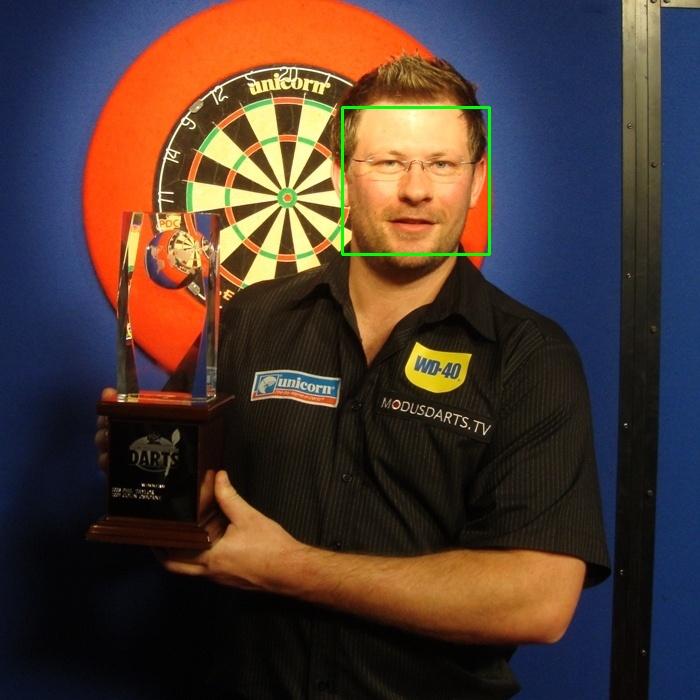
\includegraphics[width=.9\linewidth]{images/detected0.jpg}
  \caption{darts4.jpg}
  \label{fig:sub1}
\end{subfigure}%
\begin{subfigure}{.5\linewidth}
  \centering
  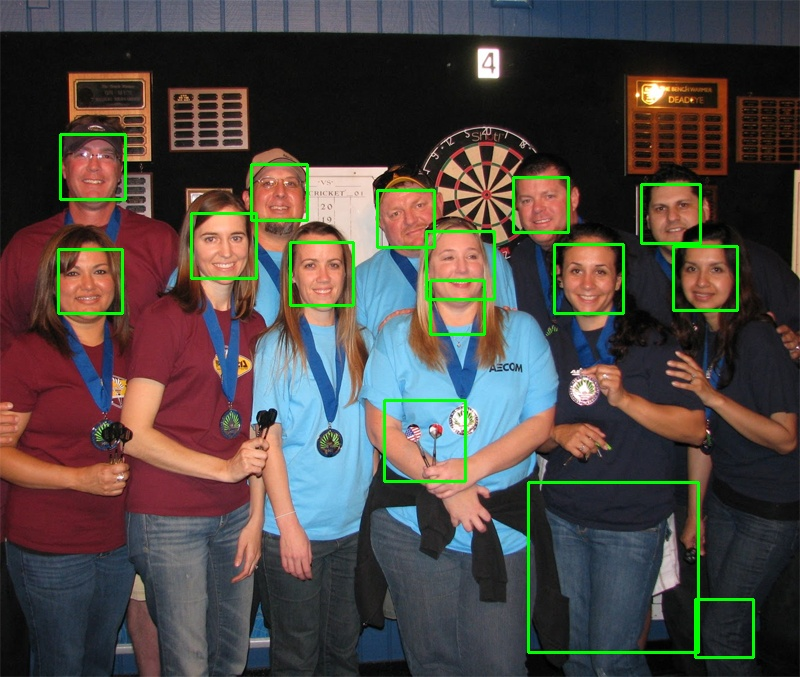
\includegraphics[width=.9\linewidth]{images/detected1.jpg}
  \caption{darts5.jpg}
  \label{fig:sub2}
\end{subfigure}

\begin{subfigure}{.5\linewidth}
  \centering
  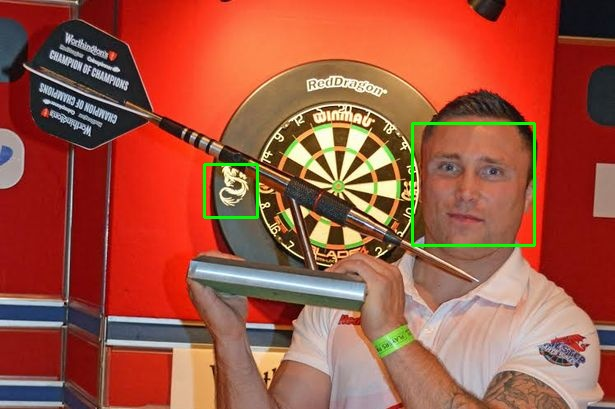
\includegraphics[width=.9\linewidth]{images/detected2.jpg}
  \caption{darts13.jpg}
  \label{fig:sub1}
\end{subfigure}%
\begin{subfigure}{.5\linewidth}
  \centering
  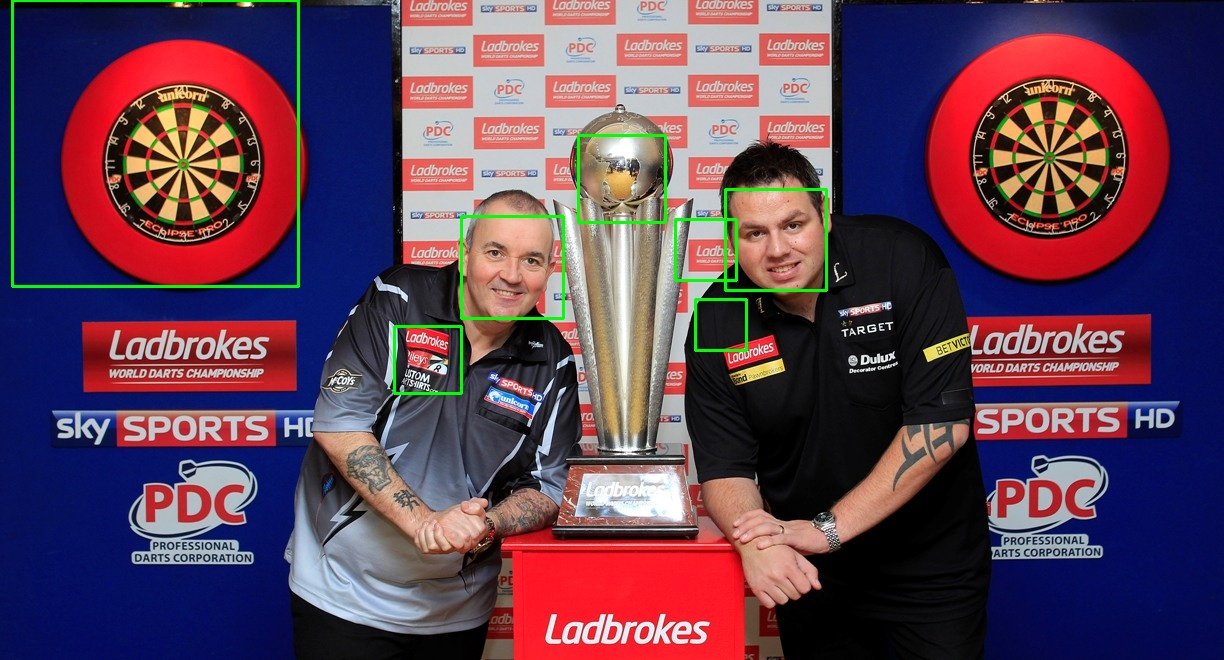
\includegraphics[width=.9\linewidth]{images/detected3.jpg}
  \caption{darts14.jpg}
  \label{fig:sub2}
\end{subfigure}


\begin{subfigure}{.5\linewidth}
\centering
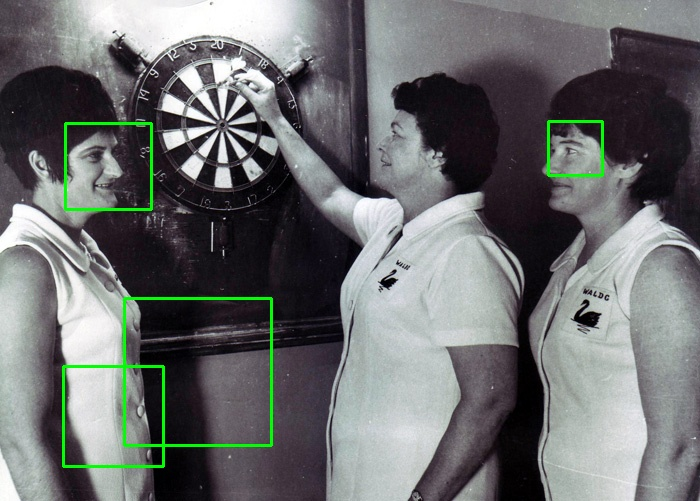
\includegraphics[width=0.9\linewidth]{images/detected4.jpg}
\caption{darts15.jpg}
\end{subfigure}


\caption{Five images with the applied face detection algorithm.}
\label{fig:q13}
\end{figure}

\subsection{Subtask b}
\subsubsection{}
TPR is difficult to assess because...
\subsubsection{}
It is always possible to get a 100 per cent detection rate on any classification task as we can select all possible areas of an image, regardless if they contain a target or not. The key to a good classifier is to get a high true positive rate, whilst keeping the false positives minimal. 

\subsubsection{}
Calculate the F1 score here. 



\section{Task Two}
\subsection{Subtask a}
\begin{figure}[htbp]
\begin{center}
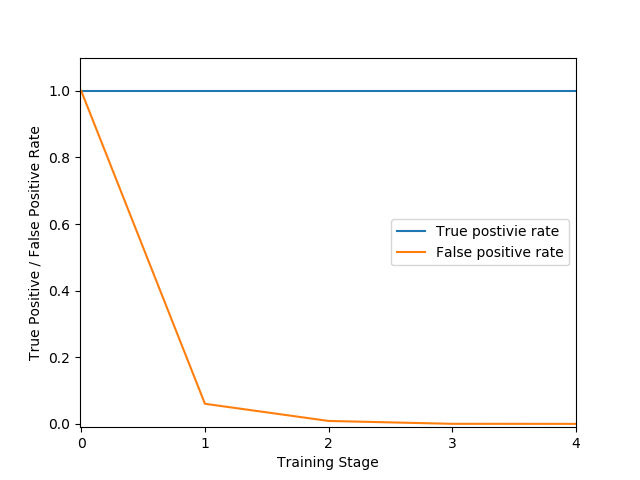
\includegraphics[width=\linewidth]{images/TPRvsFPR}
\caption{True positive rate plotted against false positive rate, when training the cascade classifier on images of dartboards. Each stage of training has been plotted as its own point.}
\label{default}
\end{center}
\end{figure}







\end{document}